%*******************************************************
%                       EINLEITUNG  
%*******************************************************
\chapter[Einleitung]{\label{sec:Einleitung}Einleitung}
% max 1 Seite
Mit den aktuellen Herausforderungen bei der Reduzierung von Treibhausgasen steigt das Interesse an Energiespeicherkonzepten, welche den Weg für energieeffiziente und nachhaltige Systeme ebnen. Besonders bei der Verwendung in mobilen Systemen, wie etwa elektrischen Fahrzeugen \cite{Huo2015,Donateo2015,Jochem2015,Kim2014,Orsi2016,Silva2011,Holdway2010,Sternberg2015,Ramachandran2015} und mobilen Robotern \cite{Hecht2023,Mikolajczyk2023,Ghobadpour2023,Wang2020}, haben sich die Vorteile von batteriebetriebenen Systemen gezeigt.

Herkömmliche Batterien sind oft nur wenig mechanisch belastbar, weshalb sie häufig mit einer zusätzlichen Schutzstruktur umgeben sind. Hinzukommt, dass durch die klare Funktionsteilung keine synergetischen Effekte genutzt werden können, wie z.B. bei Materialien, die sowohl als Energiespeicher als auch als Strukturkomponente dienen können. Das daraus resultierende niedrige Energiespeicher-zu-Masse-Verhältnis des Gesamtsystems ist eine der größten Schwächen dieser Technologie \cite{Armand2020,Schaefer2018,Cano2018,Goodenough2009}.
So nehmen die Materialien, die keinen Beitrag zur Energiespeicherung leisten, einen Massenanteil von etwa 40~\% in der von Audi Q4 e-tron Reihe eingebauten Batteriepacks ein \cite{Radu2021,Audi2022}, siehe Anhang~\ref{ch:AudiEnergie}. %Gesamtenergiedichte von 37~kWh/kg. Der Grenzwert für den Nutzen im Bereich des elektrischen Fliegens liegt nach \textsc{Scholz et al.} bei 51.8~Wh/kg \cite{Scholz2018}.

Ein vielversprechender Ansatz ist dabei die Entwicklung von sogenannten Struktur-Batterien, die zusätzlich zu ihrer Speicherfunktion auch lasttragend sein können \cite{Johannisson2018,Danzi2021,Wetzel2004, Thomas2004,Liu2009,Ekstedt2010,Wang2019,Asp2019, Moyer2020,Zhao2020, Yin2020,Wang2020,Lutkenhaus2020,Fu2021,Jin2021,Kalnaus2021,Wong2007,Carlson2013,Xu2022} und damit signifikante Einsparungen bei der Gesamtmasse und dem Gesamtvolumen ermöglichen \cite{Wetzel2004,Snyder2015,Carlstedt2020a,Asp2014,Johannisson2019}. Diese haben zudem den Vorteil, dass sie sich leichter in bestehende Designs integrieren lassen, was die Gewichtsverteilung erleichtern und einen Einbau näher am Verbraucher ermöglichen kann, wodurch Kabel eingespart werden. Diese Vorteile erlauben neue innovative Designs im Bereich Elektrofahrzeuge, elektrische Alltagsgeräte wie etwa Laptops und Telefone, mobile Roboter, Flugdrohnen und Satelliten.

Diese Dissertation fokussiert sich auf die computergestützte Suche von Struktur-Batterien in laminarer Bauweise.

Die hier dargestellte Forschung ist Teil der vom Deutschen Bundestag geförderten Forschungsinitiative „Luftfahrtforschung und -technologie“ LuFo-VI-2 in der Programmlinie „(A) Disruptive Technologien und innovative Systeme (ökoeffizientes Fliegen)“ im Fachbereich „(4) Strukturen und Bauweisen“ mit dem wichtigsten förderpolitischen Ziel „umweltfreundliche Luftfahrt“. Dies geschieht im Rahmen der „Entwicklung und Erprobung ultraleichter Verbundstrukturen mit integrierter elektrischer Speicherfunktion“ (ElViS).


%*************************************************************
%               Motivation und Zielstellung  
%*************************************************************
\section{\label{sec:Motivation_Zielstellung}Problemstellung und Zielsetzung}
% rund 1,5 Seiten inklusive Bild

%Um die Reichweite und Nutzungsdauer von mobilen elektrischen Geräten, wie Elektrofahrzeuge und mobile Roboter zu erhöhen ist sind elektrische Speicher mit besserem Verhältnis von Speichervermögen zu Gesamtmasse von entscheidenter Bedeutung. Aus dieser übergeordneten Zielstellung leiten sich drei mögliche Ansätze ab: erstens die Energiedichte der einzelnen Speicherzellen steigern, zweitens die Masse der mechansichen Entkoppelung durch die Verwendung von Werkstoffen mit hoher spezifischer Festigkeit und Steifigkeit reduzieren und drittens die Erhöhung der Gesamtenergiedichte durch die Verwendung von mechanisch belastbaren Batterien, welches einen Kompromiss zu den ersten beiden Ansätzten darstellt.

%Der letzte Ansatz hat außerdem den Vorteil, dass solche strukturtragenden Batterien (kurz Strukturbatterien) flexibler verbaut werden können und somit bei Verkabelung eingespart werden kann und Gewichtsverteilungsprobleme, wie sie etwa bei Flugmaschinen und Satelliten auftreten einfacher gelöst werden können

Derzeitige Strukturbatterien zeichnen sich oft durch eine große mechanische Steifigkeit und eine verhältnismäßig geringe Energiedichte aus. Dies macht sie jedoch für die meisten primären Anwendungsfälle ungeeignet und beschränkt damit ihr Anwendungsfeld auf sekundäre oder Schwachstromanwendungen (\textit{engl.} low energy applications). Der Mangel an Strukturspeichern mit signifikant höheren Energiedichten stellt neben weiteren ungeklärten Fragestellungen zum Austausch und Recycling eine Markteintrittsbarriere dar.

Hinzu kommt, dass die bisherige Forschung in diesem Bereich sich hauptsächlich auf die Untersuchung und Verbesserung einzelner Komponenten wie Strukturelektrolyte und den Bau spezifischer Konfigurationen konzentriert. Dabei wurde jedoch eine ganzheitliche Methodik zur Verknüpfung der Erkenntnisse aus den verschiedenen Teilbereichen vernachlässigt. So lässt sich aktuell nur schwer bewerten, inwiefern ein neues Material, das bessere elektrochemische Eigenschaften, aber schlechtere mechanische Eigenschaften als ein beliebiges Referenzmaterial hat, nun besser oder schlechter für den Einsatz in Strukturbatterien geeignet ist. Zudem basiert die Forschungsmethodik größtenteils auf experimentellen Ansätzen und wenigen computergestützten Modellen. Diese sind oft rechenintensiv und erfordern auf niedrigen Skalen den Einsatz von Supercomputern. Des Weiteren benötigen die existierenden physikalischen Modelle eine Vielzahl an Materialkennwerten, die teilweise sehr aufwendig bestimmt werden müssen.

\begin{figure}[ht]
	%\raggedleft
		%\def\svgwidth{\columnwidth}
        \center
	\includegraphics[width=\textwidth, angle=0]{motivation.pdf}
		\caption{\label{fig:motivation} Durch Strukturbatterien könnten a) eine Vielzahl an Anwendungen profitieren. Aktuelle Strukturbatterien zeigen jedoch noch viel ungenutztes Potenzial bei den elektrochemischen Eigenschaften, wie etwa Energiedichte.}
\end{figure}

Diese Dissertation zielt darauf ab, die bestehende Lücke durch die Entwicklung einer digitalen Methode zu schließen. Diese Methode soll helfen, den experimentellen Aufwand zu reduzieren und Neuerungen im wissenschaftlichen Bereich besser zu berücksichtigen und einzuschätzen. Die Methodik muss in der Lage sein, sowohl Daten aus der vorhandenen Literatur als auch aus eigenen Experimenten zu nutzen, um qualitative Aussagen über mögliche Strukturbatterievarianten für eine Vielzahl anwendungsgetriebener Fragestellungen zu treffen.

Der Ausgangspunkt ist die Erarbeitung einer modellgetriebenen Auslegung, erweitert um die Bewertung fehlender Teilaspekte. Der erste Schritt ist die Erstellung einer Materialdatenbank für mögliche Strukturbatterieanwendungen, was auch die Recherche von Materialkandidaten aus dem Bereich Leichtbau und aktueller Batterieforschung einschließt. Die hierbei ermittelten Parameter dienen als Datengrundlage für den zweiten Schritt. In diesem Schritt werden existierende computergestützte Modelle verknüpft und mit eigenen Modellen erweitert. Die eigenen Modelle werden mit Daten aus der Literatur und Experimenten, die während des Projektzeitraums ElViS stattfanden, einzeln validiert. Im dritten Schritt werden potenzielle Strukturspeicher mithilfe der validierten Einzelmodelle bewertet und exemplarisch an ausgewählten Kandidaten überprüft. Die ermittelten vorteilhaften Parameterkombinationen dienten \textsc{Kühn} und \textsc{Seidel-Greif} als Grundlage für ihre experimentellen Untersuchungen, die in der prototypischen Fertigung einer Strukturbatterie kulminierten.

Mithilfe der entwickelten Methode konnte eine optimierte Strukturbatterie für einen hybriden Anwendungsfall identifiziert werden. Ein erster Funktionsprototyp zeigte eine xx~\% höhere multifunktionale Performanz gegenüber bisher veröffentlichten Strukturbatterien.

% Das zugrundeliegende Prinzip dieses Lösungsansatzes besteht darin, dass Computer besser dazu geeignet sind, eine Vielzahl von einfachen Zusammenhängen zu verarbeiten und dies wiederholt für jede erdenkliche Kombination anzuwenden. Im Gegensatz zu bestehenden Ansätzen beginnt die Modellierung nicht auf atomarer Ebene, sondern auf der Komponentenebene, was eine schnellere Generierung von Ergebnissen ermöglicht. Zudem kann das Modellsystem leicht um Modelle auf mikro- oder molekularer Ebene erweitert werden, um zusätzliche Einflussfaktoren zu berücksichtigen.


%**************************************************************
%                   LITERATURÜBERSICHT  
%**************************************************************
\section{\label{sec:Literaturübersicht}Literaturübersicht}
% 3-5 Seiten

\subsection{Exitierende Strukturbatteriekonzepte}

\begin{figure}[ht]
	%\raggedleft
		%\def\svgwidth{\columnwidth}
        \center
	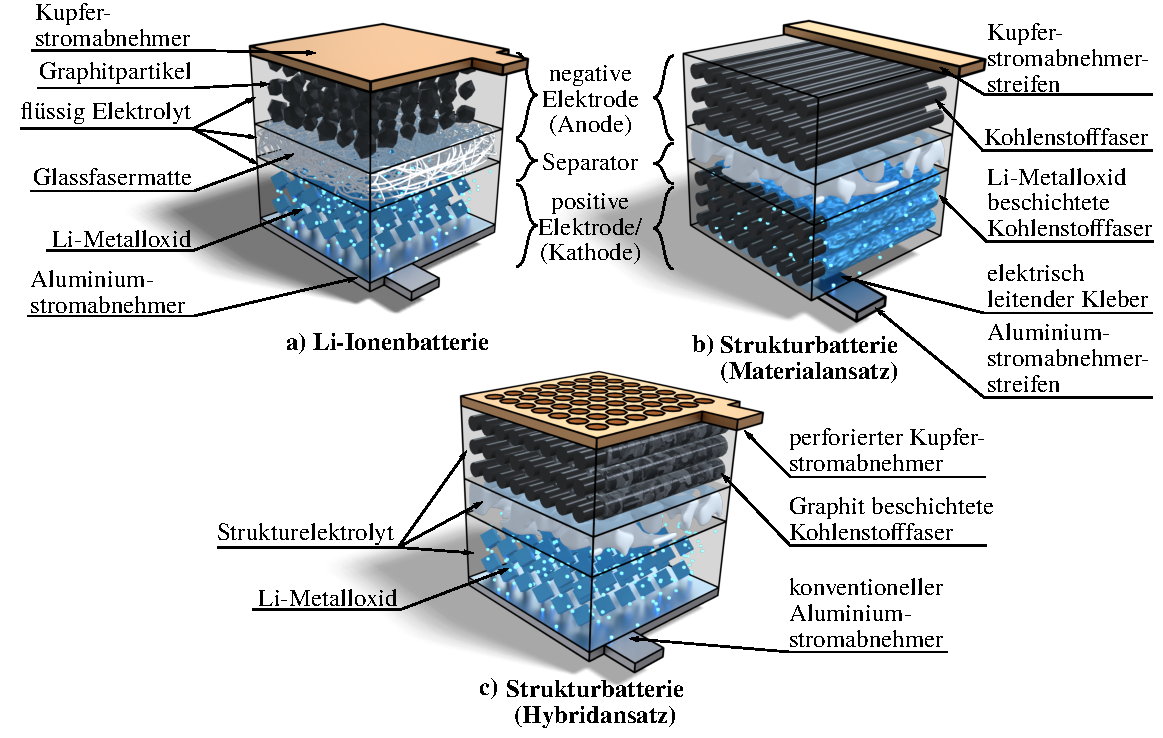
\includegraphics[width=\textwidth, angle=0]{sb_types.pdf}
		\caption{\label{fig:sb_types}Vereinfachte Darstellung von a) konventionellen Li-Ionen Batterie, b) einer Strukturbatterie als multifunktionales Material und c) als multifunktionale Struktur.}
\end{figure}

Die erste multifunktionale Strukturbatterie wurde 2004 von \textsc{Wetzel et al.} im Army Research Laboratories (ARL) der USA entwickelt \cite{Wetzel2004, Snyder2006, Wong2007, Snyder2007}. Dieses Strukturbatterieverbundmaterial basierte auf Kohlenstofffasern als Anode, einer mit $\text{LiFePO}_\text{4}$ beschichteten Edelstahlkathode und einer Glasfasermatte als Separator \cite{Wong2007}. Dieser Aufbau zeigte bereits gute mechanische Eigenschaften. Allerdings konnten die elektrochemischen Eigenschaften wegen auftretender Kurzschlüsse nicht abschließend bestimmt werden.

2009 konzeptionierten \textsc{Liu et al.} \cite{Liu2009} die erste Kurzfaser-verstärkte Elektrode mit einem festen Polymerelektrolyten als Matrixmaterial. Allerdings konnte das Team die faserverstärkte Elektrode nicht herstellen oder einen Feststoffelektrolyten mit ausreichender Ionenleitfähigkeit finden, weshalb schließlich auf ein gelbasiertes Elektrolyt mit festen und flüssigen Phasenanteilen umgeschwenkt wurde. Da aufgrund der besseren Ionenleitfähigkeit weniger Elektrolyt eingesetzt werden musste, konnte eine Energiedichte von 35~Wh/kg erreicht werden. Durch die fehlende strukturelle Verstärkung wurde allerdings nur eine geringe Zugsteifigkeit von 3~GPa erreicht.

Der Ansatz des Gelelektrolyten wurde von \textsc{Ekstedt et al.} aufgenommen \cite{Ekstedt2010}, die erstmals ein Kohlenstofffasergewebe einbetteten. Ähnlich wie in den Arbeiten von \textsc{Wetzel et al.} wurde auch hier ein glasfaserbasierter Separator und eine mit $\text{LiFePO}_\text{4}$ beschichtete, gewebte Aluminiumfasermatte als Kathode verwendet. Die resultierende Batterie zeichnete sich durch eine Zellspannung von 3,3~V aus. Allerdings wurden die mechanischen und elektrochemischen Eigenschaften nur theoretisch ermittelt.

Im Jahr 2011 präsentierten \textsc{Carlson et al.} \cite{Carlson2011} eine der ersten funktionierenden Strukturbatterien mit einer laminatartigen Struktur. Diese bestand aus einem IMS65-Kohlenstofffaserngewebe als Anode, einem Gelelektrolyt, einem Glasfaserseparator und einer mit $\text{LiFePO}_\text{4}$ beschichteten gewebten Aluminiumfolie. Die speicherbare elektrische Energie betrug 0,0247Wh/kg, was ausreichte, um eine LED 70~s lang zum Glimmen zu bringen.

Zwei Jahre später wurden \textsc{Asp et al.} \cite{Asp2013US,Asp2013CN} zwei Patente zugesprochen, die einen Ansatz beschreiben, durch gezielte Funktionalisierung der Faseroberflächen jede Kohlenstofffaser zu einer Elektrode zu machen. Auch wenn die Patente seit 2017 nicht mehr verfolgt werden, wurde darauf aufbauend eine Batterie entwickelt, mit der eine Energiedichte von 10~Wh/kg erzielt wurde. Die theoretisch möglichen 175~Wh/kg bei einem gleichzeitigen Schubmodul von 1~GPa wurden jedoch noch nicht ansatzweise erreicht \cite{Leijonmarck2013, Carlson2013}.

2018 untersuchte \textsc{Meng et al.} \cite{Meng2018} erstmalig den Einsatz von vertikal ausgerichteten Karbonnanoröhren (CNT). Diese wurden für die Elektrode auf ein Edelstahlnetz aufgedampft. Anschließend wurde für die Anode $\text{NiO}_\text{x}$ durch einen elektrochemischen Ausscheidungsprozess aufgebracht. Mit dem gleichen Verfahren wurde $\text{FeO}_\text{x}$ für die Kathode auf die CNT-Edelstahlelektrode eingelagert. Die Strukturbatterie erreichte dabei eine Zugsteifigkeit von 7,0~GPa und eine Energiedichte von 1.4~Wh/kg.

\textsc{Moyer et al.} \cite{Moyer2020} modifizierten den für Batterien typischen Pouchzellenansatz, indem das verpresste Kohlenstofffasergewebe als Stromkollektor und Schutzfolie dient. Durch das anodenseitige Aufbringen von Graphit und $\text{LiFePO}_\text{4}$ auf der Kathode nehmen die Fasern jedoch nicht direkt am chemischen Prozess teil. Durch das bessere Interkalationsverhalten bei Graphit konnte eine hohe Energiedichte von 35~Wh/kg gemessen werden. Jedoch führte der Ansatz zu einer vergleichsweise geringen Zugsteifigkeit von 2~GPa.

\textsc{Thakur et Dong} \cite{Thakur2020} stellten 2020 die erste 3D-gedruckte Strukturbatterie her. Mithilfe eines Koextrusionsprozesses konnte eine Kohlenstofffaser, die vorher mit einem festen Polymerelektrolyten beschichtet wurde, zusammen mit einem Li-gedopten Matrixmaterial aufgebracht werden. Nach dem Drucken der Elektrode wurde manuell eine Glasfasermatte und abschließend eine Aluminiumfolie als Gegenelektrode aufgebracht. Neben der Möglichkeit, neue Batterieformen zu drucken, wurde auch durch die höhere Dichte an Aktivmaterial in Fasernähe eine vergleichsweise hohe Energiedichte von 24~Wh/kg erreicht. Allerdings konnte durch den geringen Faservolumenanteil ein niedriges Zugmodul von 0.29~GPa gemessen werden.

2021 präsentierte \textsc{Asp et al.} \cite{Asp2021} ein Design mit unidirektionalen Kohlenstofffasern als Anode, einem gewebten Glasfaserseparator und einer $\text{LiFePO}_\text{4}$-beschichteten Aluminiumplatte als Kathode. Durch ein verbessertes Herstellungsverfahren und eine günstige Faseranordnung konnte eine Zugsteifigkeit von 25GPa und eine Zugfestigkeit von 300MPa gemessen werden. Gleichzeitig erreichte die Strukturbatterie eine Energiedichte von 24~Wh/kg. \textsc{Siraj et al.} \cite{Siraj2023} verbesserten zwei Jahre später den Infiltrationsprozess, wodurch sie bei annähernd gleichbleibenden mechanischen Eigenschaften die Energiedichte nahezu verdoppeln konnten, auf 41~Wh/kg.

\begin{table}[ht]
    \centering
    \caption{Auswahl realisierter Strukturbatterien}
    \begin{tabular}[t]{m{0.15\textwidth} m{0.15\textwidth}<{\centering} m{0.15\textwidth}<{\centering} m{0.2\textwidth}<{\centering} m{0.1\textwidth}<{\centering} m{0.1\textwidth}<{\centering}}
    \toprule
    &Elastizitäts-modul~[GPa]&Energie-dichte~[Wh/kg]&Struktur-batterieart&Jahr&Referenz\\
    \midrule
    \textsc{Wong et al.}&8&/&Edelstahlbatterie&2007&\cite{Wong2007}\\
    \textsc{Liu et al.}&3&35&Faserbatterie&2009&\cite{Liu2009}\\
    \textsc{Meng et al.}&7&4&Edelstahlelektroden&2018&\cite{Meng2018}\\
    \textsc{Moyer et al.}&35&2&Kohlenstofffaser-verbund&2020&\cite{Moyer2020}\\
    \textsc{Thakur et Dong}&0.29&24&Faserbatterie&2020&\cite{Thakur2020}\\
    \textsc{Huang et al.}&9.2&43&Edelstahlelektroden&2020&\cite{Huang2020}\\
    \textsc{Asp et al.}&25&24&Kohlenstofffaser-verbund&2021&\cite{Asp2021} \\
    \textsc{Saraj et al.}&26&41&Kohlenstofffaser-verbund&2023&\cite{Siraj2023}\\
    \bottomrule
    \end{tabular}
\end{table}%

Die existierenden Studien an Strukturbatterieverbundmaterialien zeigen eine Reihe an Verbesserungspotenzialen für weitere Forschungen. Die größte Herausforderung stellt dabei das Erzielen einer möglichst guten Lithiuminterkalation in das Aktivmaterial der Elektrode und unbehinderten Lithiummigration zwischen diesen dar, bei gleichzeitiger Beibehaltung der mechanischen Steifigkeit und Festigkeit \cite{Asp2015}. Auch ist die aktuell höchste erreichte Energiedichte von 35~Wh/kg am unteren Ende der benötigten Energiedichte, die für den Einsatz in z.B. Elektrofahrzeugen erforderlich ist. Diese minimale Einstiegsgrenze wurde allerdings 2022 von dem Forschungsteam von \textsc{Linde} am Deutschen Luft- und Raumfahrtzentrum (DLR) weiter angehoben und befindet sich nun eher bei einer Energiedichte von 74~Wh/kg, mit einem Zugmodul und einer Festigkeit von 54~GPa bzw. 203~MPa sowie einer Leistungsdichte von 376~W/kg \cite{Ishfaq2022}.

\subsection{Beschreibung des elektrochemischen und mechanischen Verhaltens von Strukturbatterien}

Eine der größten Herausforderungen bei der Entwicklung neuer Strukturbatterien besteht in der Beachtung aller auftretenden Wechselwirkungen, die durch den hohen Multifunktionalitätsgrad von Material und Struktur entstehen.

Eine vergleichsweise einfache Beschreibung der elektrochemischen und thermischen Prozesse kann durch äquivalente Ersatzschaltungen (\textit{engl.} equivalent circuit model, ECM) erfolgen \cite{Bavsic2022}. Bereits mit wenigen Elementen lassen sich Spannungsänderungen in Abhängigkeit vom Lade- und Entladeverhalten gut annähern \cite{YannLiaw2004}. Durch zusätzliche Erweiterungen lassen sich auch Alterung und der Einfluss zahlreicher thermischer Effekte berücksichtigen \cite{Hannan2017,Tran2021}. Aufgrund des geringen Rechenaufwands eignen sich diese Modelle besonders gut für zeitkritische Anwendungen wie die Lade- und Entladeregelung, siehe Abbildung~\ref{fig:battery_modelling_in_context}. Die Modellparameter müssen jedoch jedes Mal durch einen Fittingprozess für das jeweilige System bestimmt werden \cite{Tomasov2019}. Eine Verknüpfung der einzelnen Schaltelemente mit realphysikalischen Größen war bisher nur wenig erfolgreich \cite{Plett2015}.
\begin{figure}[ht]
	%\raggedleft
		%\def\svgwidth{\columnwidth}
        \center
	\includegraphics[width=\textwidth, angle=0]{batterie_modelling_approaches.pdf}
		\caption{\label{fig:battery_modelling_in_context}Übersicht der Batteriemodellierung im Kontext neuer Batterieentwicklungen.}
\end{figure}
Die physikalische Modellierung der elektrochemischen Prozesse wurde maßgeblich von \textsc{Doyle} \cite{Doyle1995,Doyle2003,Ceder2002}, \textsc{Fuller} \cite{Fuller2018,Takeuchi2008} und \textsc{Newman} \cite{Doyle1995,Newman2021} vorangetrieben. Das von ihnen entwickelte und nach ihnen benannte DFN-Modell (alternativ auch \textit{pseudo zwei dimensionale} (P2D) Modell genannt) \cite{Doyle1993} beschreibt die Prozesse auf der Makroskala und eignet sich daher sehr gut, um die Vorgänge auf Zellebene zu modellieren. Die benötigten Parameter können durch Experimente oder mithilfe von Simulationen auf niedrigeren Skalen wie der Dichtefunktionaltheorie (DFT) oder molekulardynamischen (MD) Simulationen bestimmt werden \cite{Chen2022}. Das DFN-Modell findet heute weitreichenden Einsatz und wurde seit seiner Veröffentlichung im Jahr 1993 zahlreich modifiziert und erweitert. Einige der bekanntesten Derivate sind das \textit{Single Particle Model} (SPM) \cite{Li2017} und das \textit{full homogenized macro-scale} (FHM) Modell \cite{Arunachalam2019}, welche beide darauf abzielen, die sehr rechenintensiven Differentialgleichungen in ihrer Komplexität zu reduzieren.

Die Kopplung mit thermischen Prozessen wurde bereits 1995 von \textsc{Pals et Newman} \cite{Pals1995,Pals1995a} begonnen und seitdem kontinuierlich weiterentwickelt \cite{Chen2005,Onda2006,Kim2013,Gao2021,Liu2023}. Auch der Einfluss der lithierungsbedingten Ausdehnung \cite{Bower2011,Yang2014,Roberts2014,Pereira2019,Mai2019,Li2020,Hoeschele2023}, Rissbildung \cite{Dionisi2017,Wang2020a,Pistorio2023} und Alterung \cite{RedondoIglesias2020} wurden in zahlreichen Studien untersucht. Zusätzlich existieren viele Studien, die sich einer vereinheitlichten Modellierung aller Effekte \cite{Wu2014,Kim2018,Liu2020,Yin2020} und auch einer Modellierung über mehrere Größenskalen hinweg widmen \cite{Liu2019,Li2020a,Katrasnik2021}.

\textsc{Carlstedt} erarbeitete stückweise in einer Reihe von Beiträgen eine Koppelung von Elektrochemie, Mechanik und Thermodynamik, um das Verhalten von Strukturbatterien zu beschreiben \cite{Carlstedt2019,Carlstedt2019a,Carlstedt2019b,Carlstedt2020,Carlstedt2020b,Carlstedt2022,Carlstedt2022a,Carlstedt2022b}. Auch wurde der Ansatz um den nicht-linearen Zusammenhang durch die Gestaltänderung von \textsc{Larsson et al.} \cite{Larsson2023} erweitert.

\subsection{Modelierungsgetriebene Entwicklung von neuen Batterien und Strukturbatterien}

Die neu motivierte Forschung in bereits untersuchte und neue Batteriematerialien baut aktuell hauptsächlich auf theoretischen Überlegungen und experimentellen Prototypen auf. Um die Vielzahl an Effekten zu berücksichtigen und der enormen Anzahl an vielversprechenden Materialkombinationen Herr zu werden, argumentierten \textsc{Greenhalgh} \cite{Greenhalgh2024,Greenhalgh2024a} und \textsc{Asp} \cite{Asp2024} auf dem \textsc{1st Structural Power Research Showcase} in London, dass nur durch intensive Modellierungsarbeit diese Varianten voruntersucht und ausreichend eingeschränkt werden können. Der multiphysikalische Modellierungsansatz von \textsc{Carlstedt} wird zwar in diesem Zusammenhang oft erwähnt, allerdings sorgen Skalierungseffekte, wie etwa Defekte und Faser-Matrix-Interfaceeffekte, die besonders bei Oberflächenmodifikation von Kohlenstofffasern sowohl für deutlich andere elektrochemische als auch mechanische Eigenschaften des Verbundes sorgen, für große Ungenauigkeiten bei der Adaption \cite{Franco2019,Fam2024}. Hinzu kommt, dass die Modelle von Carlstedt mit zunehmender Komplexität immer mehr Materialparameter benötigen und bereits jetzt mehr als 20 teils aufwendig zu bestimmende Parameter pro Material erfordern \cite{Greenhalgh2024a}. Bis heute wurde dieser Ansatz daher vor allem zur nachträglichen Validierung und zur detaillierten Untersuchung von sensorischen und aktuatorischen Effekten von Strukturbatterien genutzt \cite{Carlstedt2023}.

Die einzige zurzeit existierende Veröffentlichung zur Vorhersage von Energiedichte und Zugsteifigkeit stammt ebenfalls von \textsc{Carlstedt} \cite{Carlstedt2018}. Jedoch wurde dazu ein in der Komplexität deutlich reduzierter Ansatz verwendet. Hinzu kommt, dass bei der Auswertung nur drei Varianten untersucht wurden, die sich in ihrer Elektrodendicke und dem Volumenanteil des Aktivmaterials unterschieden. Außerdem wurde der Einfluss des Elektrolyten nicht berücksichtigt.



% Dan Zenkert KTH Prof (Fasercehmie), 
% Dr Faye Smith OBE (Director at Avalon Consultancy Services)
% Peter Linde (DLR, CORCER Mitgleid)
% Milo Shaffer ( Professor of Materials Chemistry London)
% Natasha Shirshova (Lecturer in Engineering Materials at Durham University)
% Derrick Fam (Scientist at Institute of Materials Research and Engineering (IMRE), Adjunct Assistant Professor (NTU, MSE), Dy. Dir. Singapore Battery Consortium)
% Alexander Bismarck (Professor of Material Chemistry Wien)
% Madhavi Srinivasan (Professor at Nanyang Technological University Singapore)



   

